%%%% --------------------------------------------------------------------------
%%
%%          K I L O N O V A
%%
%%%% --------------------------------------------------------------------------

\chapter{Kilonova} \label{ch:kilonova} 

In this chapter we discuss models of the quasi-thermal counterpart 
of the \ac{BNS} mergers, powered by the decay of the newly sythesized heavy 
elements via \rproc{} \nuc{} discussed in the previous chapter \ref{ch:nucleo}.
%
In Sec.~\ref{sec:intro:kilonova} we recall the origin of the quasi-thermal emission, 
the energy release in nuclear heating, its thermalization in ejecta, and the 
opacities of the latter and how they shape the final emission giving a unique 
signature. 
%
In the Sec.~\ref{sec:kilonova:albino} we describe the model, 
developed by \cite{Perego:2017wtu}, that was used in this thesis to 
produce synthetic light curves. Finally, in Sec.~\ref{sec:kilonova:result} 
we report the results of our analysis.

%% --------------------------
%% M O D E L L I N G  K I L O N O V A
%% --------------------------

%The \rproc{} \nuc{} in ejecta is primarily determined by the electron fraction 
%\citep{Lippuner:2015gwa}, $Y_e$, producing $3$rd ($1$st) elements of the \rproc{} peaks 
%%(See Sec.~\ref{sec:intro:nucleo}) 
%if the $Y_e\gtrsim 0.3$ ($Y_e \lesssim 0.2$) 
%with respective abundances in the former remarkably close to solar. 
%%The transition at $Y_e{\simeq}0.25$ is rather sharp.



\subsection{Overview of kilonova modelling} \label{sec:intro:kilonova}

\citet{Li:1998bw} suggested that 
radioactive decay of the material enriched with \rproc{} elements,
ejected in \ac{BNS} or \ac{NSBH} mergers,
can power an \ac{EM} transient.
%
Authors showed that contrary to the normal \acp{SN}, 
the ejecta would quickly become transparent to its own emission, peaking on a timescale 
of around a few days. 
%
The main difficulty in this pioneering work was the lack of a \nuc{}
models to estimate the radioactive heating in the ejecta. 
%
The understanding of \ac{kN} has significantly improved since then
\citep[\eg][]{Kulkarni:2005jw,Metzger:2010,Roberts:2011,Metzger:2016pju,Wollaeger:2017ahm} 
and advanced even further with the detection of \AT{} \citep[\eg][]{Metzger:2019zeh}.


The way to compute \ac{EM} emission from stratified, asymmetric ejecta is to perform 
multi-dimensional, multi-group radiative transfer simulation coupled to \ac{HD} (or \ac{MHD}) 
simulation of the ejecta itself \citep[\eg][]{Bulla:2019muo}.
%
It is however possible to compute the bolometric\footnote{
    Related to the total emitted radiation at all wavelengths. 
} properties considering the total amount 
of energy released and emitted by radioactive decay within ejecta. 

%
%Here a simplified model is considered of a transient, powered by the radioactive decay 
%within the ejecta only. Several other assumptions are made. In particular, the ejecta 
%expansion is homologous (faster matter ahead of slow one) \citep{Rosswog:2013kqa}. %%{(Rosswog et al 2014)}
%
%\red{this is based on the Barnes PhD thesis on Opacities for Kilonva (Rad.Transport)}
%\red{Based on Metzger paper }

%% --------------------------
%% SIMPLE MODEL
%% --------------------------

%\subsubsection{Basic ingredients}

%Consider the following simplified approach to compute the \ac{EM} signal from \rproc{}
%elements enriched material. 
Let the radioactive decay of a newly synthesized heavy isotope, $i$, release 
$\dot{Q}_i \propto \exp(-t/\tau_i)$ energy, with $\tau_i$ being its half-life.
Then, assuming equal distribution of $\tau_i$ per logarithmic time, 
%(at any $t$ the dominant species have $\tau\sim t$), 
the heating rate of the ejecta at time $t$ is 
$\dot{Q}_{LP} = f M c^2 / t$,
where $f$ is the free parameter and $M$ is the ejecta mass\footnote{
    In general heating is time-dependent as thermodynamic histories of the expanding 
    ejecta (from \ac{NR} simulations) showed \citep{Metzger:2010,Roberts:2011,Korobkin:2012uy}.
    See also \citet{Hotokezaka:2017dbk} for the discussion on physical principles behind the decay.
}.
%
%In addition, provided by \citet{Li:1998bw}, normalization $f$ resulted in overestimation of the peak 
%luminosity of the \ac{kN}, that plagued the \ac{kN} searches for a decade 
%\cite{Rosswog:2005su,Dong:2015oea,Bloom:2005qx,Kocevski:2009gv}. 

The first self-consistent estimation of the heating rates based on the \ac{NRN} 
calculations of the \rproc{} in the ejecta, were carried out by the \citet{Metzger:2010}. 
The authors showed, that based only on dynamical ejecta, the \ac{EM} transient is ${\sim}10^3$ 
times brighter then Novae -- hence, the term, kilonova was coined. 
%
%It was also shown the ejecta electron fraction does not affect the heating rates
%considerably, and performed the first estimations of the thermalization 
%efficiency of decay products.
%
%The term macronova was however coind by \citet{Kulkarni:2005jw} who considered a 
%transient powered by the decay of radioactive $^{56}$Ni and free neutrons. 
%However, as it was shown later, $^{56}$Ni can only be formed in small quantities on 
%the outskirts of the ejecta.

The calculation of observed \ac{EM} emission is complicated by the %ejecta opacity, 
%as there is a 
general lack of experimental data and numerical models of the optical opacity 
of matter enriched with singly and doubly ionized heavy \rproc{} elements. 
Iron-group gray opacities were initially considered \citep{Roberts:2011}, 
but were later found to severely underestimate those of 
lanthanides and actinides with their 
complex atomic structures (given by open $f$-shells) 
\citep{Kasen:2013xka,Tanaka:2013ana}. 
%
Higher opacities shift light curve peak time by ${\sim}1\,$weak \citep{Barnes:2013wka} 
and shift the spectral peak from optical/\ac{UV} to \ac{NIR}.

%% ----------------------------------------
%\subsection{Basic model of the \ac{kN}}
%% ----------------------------------------

For a single shell of hot and optically thick matter 
(in which the thermal energy is not immediately radiated away), 
expanding with constant velocity, $\upsilon$, 
%such that $R\approx\upsilon t$ at any point in time $t$, 
the radiation diffusion timescale is given by 
%
\begin{equation}
\tau = \rho \kappa R = \frac{3}{4}\frac{M\kappa}{4\pi R^2}, \hspace{5mm} 
t_{diff} \approx \frac{R}{c}\tau = \frac{3}{4}\frac{M\kappa}{4\pi c R} = \frac{3}{4}\frac{M\kappa}{\pi c \upsilon t}\, ,
\end{equation}
%
where $M$ is the ejecta mass, $\kappa$ is the opacity (cross section per unit mass), 
$\rho$ is the density, \eg, $\rho=3M/(4\pi R^3)$ is the mean density.
%
As ejecta expands and cools (via adiabatic losses) its opacities decreases, 
and so does the diffusion timescale. 
When $t_{diff}$ reaches $t$, the radiation can escape the ejecta \citep{Arnett:1982}. 
Hence, the characteristic timescale of the peak of emitted radiation 
%
%\red{check the eq.} -- Eq.5 in Metzger
\begin{equation}
t_{peak} = \Big(\frac{3}{4\pi}\frac{1}{\beta}\frac{M\kappa}{\upsilon c}\Big)^{1/2}\, ,
\end{equation}
%
where the constant $\beta$ depends on the exact density profile of the ejecta. 
The $t_{peak}$ is of order of days for lanthanides-free and weeks for lanthanides-rich ejecta.
The peak luminosity is set by the total heating rate $\dot{Q}(t)$ within the ejecta, 
as described by the \textit{Arnett's Law} \citep{Arnett:1982}. 

%% ----------------------------------------
%\subsubsection{Emission from stratified ejecta}
%% ----------------------------------------

%Consider the ejecta with a given mass-velocity distribution, that can be approximated 
%as $M_{\upsilon} = M(\upsilon / \upsilon_0)^{-\beta}$, for $\upsilon \geq \upsilon_0$,
%where $M$ is the total mass, $\upsilon_0$ is the average, minimum velocity. 
%The parameter $\beta$ can be set to $3$ \citep{Bauswein:2013yna}. %%{(Bauswein et al 2013a)}. 
%However see \citet{Piran:2012wd}%%{Piran et al 2013} 
%for a more complex velocity profiles.
%%
%%
%The diffusion timescale defines when the radiation escapes the ejecta. For a layer with 
%$\upsilon$ and $M_{\upsilon}$ and opacity $\kappa_{\upsilon}$ it is 
%%
%\begin{equation}
%t_{d,\upsilon} \approx \frac{3}{4\pi}\frac{M_{\upsilon}\kappa_{\upsilon}}{\beta Rc} = 
%\frac{1}{4\pi}\frac{M_{\upsilon}^{4/3}\kappa_{\upsilon}}{M^{1/3}\upsilon_0 t c}
%\end{equation}
%%
%where $\beta=3$ was assumed. 
%%
%This equation implies that at time $t=t_{d,\upsilon}$ the radiation from the layer 
%$M_{\upsilon}$ peaks.
%%
%The $M_{\upsilon}(t)$ is related to the total mass of the ejecta and 
%peak time (when radiation diffuses from the entire ejecta)
%%
%\begin{equation}
%M_{\upsilon}(t) = 
%\begin{cases}
%M(t/t_{peak})^{3/2},& t<t_{peak}, \\
%M, &t>t_{peak}
%\end{cases}
%\end{equation}
%%
%where $t_{peak} = (3M\kappa / (4\pi \beta \upsilon c))^{1/2}$ with 
%$\upsilon = \upsilon_0$. \red{Did not understand}
%%
%Outer layers with $M_{\upsilon} < M$ peak first, while the deepest layers peak later but 
%set the luminosity of the whole ejecta (assuming that the the opacity is constant in the 
%ejecta. 
%%
%The radial evolution of each layer $M_{\upsilon}$ of mass $dM_{\upsilon}$ is given by 
%%
%\begin{equation}
%\frac{dR}{dt} = \upsilon,
%\end{equation}
%%
%and the layer's thermal energy changes according to 
%%
%\begin{equation}
%\label{eq:theory:mkn:energ}
%\frac{dE_{\upsilon}}{dt} = \underbracket{-\frac{E_{\upsilon}}{R_{\upsilon}} 
%    \frac{dR_{\upsilon}}{dt}}_{PdV\text{ losses}} - 
%\underbracket{L_{\upsilon}}_{\text{rad. los.}} + \underbrace{\dot{Q}}_{\text{heating sources}},
%\end{equation}
%%
%where the radiative losses take form
%%
%\begin{equation}
%L_{\upsilon} = \frac{E_{\upsilon}}{t_{d,\upsilon} + t_{lc,\upsilon}},
%\end{equation}
%%
%in which the $t_{lc,\upsilon} = R_{\upsilon}/c$ limits the energy loss to the 
%light crossing time (important for when the layer is optically thin) \red{did not understand}.
%%
%The heating sources $\dot{Q}$ include
%%
%\begin{equation}
%\dot{Q}(t) = \underbrace{\dot{Q}_{r,\upsilon}}_{\text{radioactivity}} + \underbrace{\dot{Q}_{mag}}_{\text{magnetar}} + 
%\underbrace{\dot{Q}_{fb}}_{\text{fall-bak accretion}}.
%\end{equation}
%%
%%
%Next, even though in principle the effect of radiation pressure on ejecta oughtto 
%be considered, in case where radioactive heating, total energy input 
%$\int \dot{Q}_{r,\upsilon}dt < E_{kin,0}$ of the ejecta \citep{Metzger:2010,Rosswog:2013kqa} 
%%\cite{(Metzger et al 2011; Rosswog et al 2013)}, 
%this effect can be neglected.
%Meanwhile, central engine might provide enough energy to modify the free expansion 
%model. Then the equation for the central shell velocity evolution reads 
%%
%\begin{equation}
%\label{eq:theory:mkn:velcenteng}
%\frac{d}{dt}\Bigg(\frac{M\upsilon_0^2}{2}\Bigg) = M\upsilon_0\frac{d\upsilon_0}{dt} = \frac{E_{\upsilon_0}}{R_0}\frac{dR_0}{dt}
%\end{equation}
%%
%Here, the term with $E_{\upsilon_0}$ balances the $PdV$-\textit{loss} term in the 
%thermal energy equation (for $dE_{\upsilon}/dt$)
%%
%To compute the emitted radiation, first assume the black-body emission, 
%the thermal emission, with effective temperature 
%%
%\begin{equation}
%T_{eff} = \Bigg(\frac{L_{tot}}{4 \pi \sigma R_{ph}^2}\Bigg)^{1/4}
%\end{equation}
%%
%where $L_{tot} = \sum(L_{\upsilon dm_{\upsilon}})$ is the total luminosity 
%(cumulative for all mass shells). At the point where optical depth 
%$\sum(\kappa_{\upsilon}dm_{\upsilon})=1$ the photosphere is located with 
%radius $R_{ph}(t)$. 
%%
%%The flux density of the source at photon frequency $\nu$ is given by 
%%%
%%\begin{equation}
%%F_{\nu}(t) = \frac{2\pi h \nu^3}{c^2} \frac{1}{\exp\Big(\frac{h\nu}{kT_{eff}}\Big) - 1} \frac{R_{ph}^2}{D^2}
%%\end{equation}
%%%
%%where, $D$ is the distnace to the source. (Cosmological effects are neglected here).
%%
%Additionally, the opacity $\kappa_{\upsilon}$ depends on the temperature of the 
%layer $T_{\upsilon}$, that itself can be computed as 
%%
%\begin{equation}
%T_{\upsilon} = \Bigg(\frac{3E_{\upsilon}}{4\pi a R^{3}_{\upsilon}}\Bigg)^{1/4}
%\end{equation}
%%
%assuming that the ejecta internal energy is dominated by the radiation. 
%%
%%
%Finally, in order to compute the \ac{EM} emission from the ejecta, 
%the equation Eq.~\eqref{eq:theory:mkn:energ} ought be solved for $E_{\upsilon}$ 
%(and $L_{\upsilon}$) for every shell with $dM_{\upsilon}$ and $\upsilon>\upsilon_0$. 
%%
%The velocity distribution can be assumed fixed 
%(\eg $M_{\upsilon} = M(\upsilon/\upsilon_0)^{-\beta}$,  
%if only the internal heating are important. If however, the central engine energy 
%input is important, the the velocity of the central layer evolves according to
%Eq.~\eqref{eq:theory:mkn:velcenteng}.
%%
%Initial kinetic energy of the ejecta is quickly removed by the adiabatic expansion 
%and the thermal energy of the ejecta, when its emission peaks, is dominated by the heating.

%% -----------------
%% \paragraph{Opacity}
%% -----------------

In this simplified description thee key components can be identified for modeling the \ac{kN}.
These are 
%\begin{itemize}
%\item
(i) ejecta geometry and properties, $M$, $\upsilon$, $Y_e$; 
%\item 
(ii) composition of the expanding ejecta and its optical opacity; 
%\item 
(iii) dominant sources of energy within the ejecta, heating rate $\dot{Q}(t)$, and how 
efficiently this energy thermalizes.
%\end{itemize}
%
%We discuss the properties of the ejecta from \ac{BNS} mergers in the chapter~\ref{ch:bns_sims}.
%Here we focus on two other ingredients.

Regarding opacity, there are several sources of opacity that affect photons with
different energies that include 
%%%% --- free-free opacities
%For the photons of the lowest energy (frequency), \ac{FIR}, the free-free absorption 
%in the ionized gas is the dominant source of opacity. Expansion, the recombination removes 
%free $e$, also decreases $\rho$, and thus $\kappa_{ff}$.
(i) free-free transitions, especially in lanthanides and actinides with their 
valence, partially filled $f$-shell, affecting photons of lowest energies, in \ac{FIR} band; 
%%%% --- bound-bound opacities
%For \ac{NIR}/optical photons, the bound-bound transitions are the main source of opacity. 
%Here the dependency on the ejecta composition strongly affects the \textit{effective} 
%continuum opacity. If most complex atoms in the ejecta belong to the iron group, with 
%valence $d$-shell electrons, then the opacity is moderate. However, if elements with 
%valence, partially filled $f$-shell, (lanthinides \& actinides), are present, then the 
%opacity increases by up to two orders of magnitude
%\citep{Kasen:2013xka,Tanaka:2013ana,Fontes:2015,Fontes:2017zfb}. 
%Bound-bound opacity rises with photon $\nu$ (as the number of lines).
%
%The \textit{plank mean expansion opacity} can be approximated as 
%$\kappa_r = 200 (T/4000K)^{5.5}$ cm$^2$g$^{-1}$ for $T\in(1-4)\times10^3$~K and just 
%$\kappa_r = 200$ cm$^2$g$^{-1}$ for $T\in(4-10)\times10^{3}$~k, motivated by 
%Figure~10 it \citet{Kasen:2013xka}. More accurate opacity estimations are plagued by the 
%complexity of the atomic structure. The quantum mechanics models of high-$Z$ atoms exists, 
%but has to be calibrated to the so far absent experimental data.
(ii) bound-bound transitions, that are the main source of opacities for 
\ac{NIR}/optical photons, 
%%%% --- Line opacity -> Effectve continoum opacity
%Additional complexity arises in approximation the line opacities to the effective opacity.
%One common way is to consider the line expansion opacity formalism \citep{Pinto:2000}, that is 
%based on the Sobolev approximation. This method was applied to \acp{kN} modeling by 
%\citet{Barnes:2013wka} and \citet{Tanaka:2013ana}. However, it is unreliable if line width is 
%large \ie, if line spacing of strong lines become comparable to the intrinsic thermal line width 
%\citep{Kasen:2013xka,Fontes:2015,Fontes:2017zfb}. 
(iii) certain optically thick lines, broadened by relativistic effects, 
%%%% --- clumping
%In addition, clumping that might occur when $T\leq10^3$~K might affect escaping 
%emission \citep{Takami:2014oqa}. The formation of the ``\rproc{} dust'' may have a complex 
%effect on optical/\ac{UV} opacity. The process of dust formation is complex and not 
%well understood in general \citep{Cherchneff:2009sj,Lazzati:2016}
(iv) ejecta clumping, 
%%%% --- Ejecta re-ionisation
%For higher energy photos, \ac{UV}/X-ray, bound-free transitions dominate the opacity. 
%For that ejecta ought to become mostly neutral, which occures naturally as it cools, unless 
%there is a source of ionizing radiation, \eg, the remnant. 
%See for details in \eg, \citet{Metzger:2013cha}. 
%Even though very large luminocities are required from the engine initially, 
%they decrease rapidly as ejecta expands. Thus, at late times it is possible that ejecta would be 
%re-ionized, especially in case of a long-lived remnant \citep{Metzger:2013cha}. The re-ionisation 
%can reduce the optical opacity, reducing the prominence of \ac{FIR} peak, 
%a generally regarded distingushed feature of a Kilonova.
and (v) ejecta re-ionisation by \eg, high energy photons from the central engine.
%%%% --- X-ray,. Gamma-rays, thermalization
%At even higher energies, hard X-ray photons, an important source of opacity is the 
%electron scattering with Klein-Nishina corrections. Notably, if the wavelength of photons 
%become smaller then the scale of an atom, the contribution from both, free and bound into 
%nuclei electrons ought to be considered. At high energies, the scattering of photons is inelastic. 
%However, these processes are important as ejecta opacity to very high energy photons, 
%$\gamma$-rays with energy in order of MeVs, determines the thermalisation of the \rproc{} 
%decay products.
%%
%%% pair-creation
%For extremely high photon energies $h\nu \gg m_e c^2$a pair creation becomes important. 
%In particular this is so if remnant is a magnetar with large spin-down luminosity. 
%Then, the at peak of the \ac{kN} emission, the pair creation might prevent pair-creation 
%photons from escaping the kilonova. 

%The calculation of opacities is complicated by the fact that the 
%Additional complexity arises in approximation the line opacities to the effective opacity.

%%%% --- compliecations in calculations 
An additional complication in opacity calculations arises from the fact that the ejecta 
is rapidly expanding, which implies that the matter ``sees'' incoming radiation as 
Doppler shifted. 
One common approach is to consider  %\textit{plank mean expansion opacity}, 
%\red{in MKN it is mean plank opacities} 
%that for 
%$\kappa_r = 200 (T/4000K)^{5.5}$ cm$^2$g$^{-1}$ for $T\in(1-4)\times10^3$~K and just 
%$\kappa_r = 200$ cm$^2$g$^{-1}$ for $T\in(4-10)\times10^{3}$~k, motivated by 
%Figure~10 it \citet{Kasen:2013xka}.
calculation of which, however, still requires complex atomic calculations.
%
The Sobolev approximation is commonly used in the line expansion opacity formalism 
\citep{Pinto:2000}.
This method was applied to \acp{kN} modeling by \citet{Barnes:2013wka} and \citet{Tanaka:2013ana}. 
However, it is unreliable if line width is large \ie, if line spacing of strong 
lines becomes comparable to the intrinsic thermal line width 
\citep{Kasen:2013xka,Fontes:2015,Fontes:2017zfb}. 


%% ----------------------------
%% \paragraph{\rproc{} heating}
%% ----------------------------

The main source of energy in expanding ejecta shell of mass, $dM_{\upsilon}$,
and velocity, $\upsilon$, that has a fraction of \rproc{} elements, $X_{r,\upsilon}$, 
is given by the specific heating, $\dot{e}_r(t)$, and can be approximated as 
%
\begin{equation}
\dot{Q}_{r,\upsilon} = dM_{\upsilon}X_{r,\upsilon}\dot{e}_{r}(t).
\end{equation}
%
The heating occurs through a combination of $\beta$- and $\alpha$-decays, 
and fission \citep{Metzger:2010,Barnes:2016umi,Hotokezaka:2017dbk}. 
The decay products then thermalize with an efficiency, $\varepsilon_{th,\upsilon}$, 
that depends on interactions between them and thermal plasma. 
Neutrinos can freely escape the ejecta. Very high energy photos, gamma rays, 
are also free after about ${\sim}1$~day as the Klein-Nishina opacity decreases 
\citep{Hotokezaka:2017dbk,Barnes:2016umi}.
%
The $\alpha$ and $\beta$ particles however interact efficiently with the matter via 
ionization \citep{Barnes:2016umi} and Coulumb scattering \citep{Metzger:2010}.
%\red{Here it repeats the Barns et al findings on thermalization efficiency}
For a fixed energy $\alpha$-particles thermalize more efficiently, then 
$\beta$-particles. For charged particles, the process depends on the magnetic 
field strength and configuration \citep{Barnes:2016umi}. 
%
Additionally, if actinides are produced in \rproc{}, their decay, 
involving $\alpha$-particles which thermalize with high efficiency. 
%\red{double check with before, Barnes}. 
Nuclear phsyics input that determines the amount of actinides, 
have a strong effect on the thermalization efficiency of \rproc{} elements in the ejecta
\citep{Barnes:2020nfi}.
%
%For a neutron-rich ejecta, $Y_e\leq0.2$, the heating rate is dominated by a large statistical 
%ensemble of nuclei, and the following can be assumed \citep{Korobkin:2012uy},
%%
%\begin{equation}
%\dot{e}_r = 4\times 10^{18} \varepsilon_{th,\upsilon}(0.5 - \pi^{-1} \arctan[(t-t_0)/\sigma])^{1.3} \text{ erg } \text{s}^{-1} \text{g}^{-1}
%\label{eq:kilonova:heat_korob}
%\end{equation}
%%
%Here $t_0=1.3$~s, $\sigma=0.11$~s constants. 
%The $\varepsilon_{th,m}$ is the thermalisation efficiency.
%In general, both $\varepsilon_{th,\upsilon}$ and 
%%
%The heating rate prescribed by this equation has first a constant segment, $\propto1$~s, 
%(depletion of free neutrons by $r$-process) and a decrease segment $\propto t^{-1.3}$, 
%(when heavy nuclei decay to stability) \citep{Metzger:2010,Roberts:2011}. 
%Notably, at higher $Y_e$, the nuclear heating is dominated by specific nuclei and has a complex form.
%%
%It was shown however, that on a timescale relevant for \ac{kN}, and $Y_e$ present in \ac{BNS} 
%($Y_e\leq0.4$), the heating rate can be assumed constant within the accuracy of a few.
%(see \eg, Fig.~7 in \citet{Lippuner:2015gwa}).
%%
%The dependency of $\dot{Q}_{r.\upsilon}$ on the nuclear physics models was shown to be week, 
%unlike the $r$-process abundances themselves \citep{Eichler:2014kma,Wu:2016pnw,Mumpower:2015ova}.
%See however \citet{Barnes:2020nfi} for a more recent assessment.
%
%Regarding the thermalization efficiency of the energy released, \citep{Barnes:2016umi} provides 
%a recipe that sets the $\varepsilon_{th,\upsilon}$ decreasing from $\sim0.5$ at around 
%$1$~day to $\sim0.1$ at around $1$~week. 
%
%\begin{equation}
%\varepsilon_{th,\upsilon}(t) = 0.36 \Bigg[ \exp(-a_{\upsilon}, t_{day}) + \frac{\ln(1+2b_{\upsilon} 
%    t_{day}^{d_{\upsilon}})}{2b_{\upsilon}t_{day}^{d_{\upsilon}}} \Bigg]
%\end{equation}
%
%where $t_{day}$ is the time in days, ${a_{\upsilon}, b_{\upsilon}, d_{\upsilon}}$ are the constants that 
%depend on the ejecta layer properties, mass and velocity. 

%%%% -------------------------------
%\subsection{\ac{kN} properties}
%%%% -------------------------------
%
%From a simple, toy model \citep{Metzger:2016pju}, the ejecta properties can be translated 
%into the properties of light curves. 
%%
%Consider the case where the lanthanides-rich ejecta is present, \eg, in tidal outflows of 
%\ac{BNS} and \ac{NSBH} mergers. There a toy model predicts a light curve from such low-$Y_e$ 
%ejecta that peaks in \ac{NIR} (in relatively good agreement with radiation transport model of 
%\citet{Barnes:2016umi}) on a timescale of several days (week). This is so-called ``red \ac{kN}''.
%The disagreement with radiation transfer models most noticeable in the post-peak period, 
%where toy model predicts sharp decay, while the radiation transport models predict smooth decline. 
%The reason for it is the toy model's assumption of optically thick black-body emission. 
%As ejecta expands cools and become optically thin, this assumption breaks down.
%It is important to note, that the toy model does not take into account other emergent sources 
%of opacity at late times, such as clumping, dust formation, photo-ionization from central engine. 
%These may smooth the post-peak light curves.
%
%Next, consider the ejecta with high electron fraction, \eg, \nwind, or \ac{SWW}, reprocessed by neutrinos.
%Such ejecta would have negligible amount of elements of lanthanides group \citep{Metzger:2014ila} 
%and thus have a different \ac{EM} signature. The emission from such ejecta peaks in optical/\ac{IR} 
%bands on a time scale of days. It is $2-3$ magnitudes brighter then red \ac{kN}. This component is called ``blue \ac{kN}''
%This emission is assumed to be of polar origin and contribute to the total \ac{EM} signature of the BNS ejecta. 


%\subsection{Other \ac{EM} counterparts}
%\red{commented}
%\subsubsection{Free Neutron Precursor}
%
%The sufficiently high density and low veloicyt of the bulk of the ejecta assures that there is enough time for the $r$
%-process to remove free neutrons. However, a small fraction of the ejecta was shown to have hight enough velocity to retain its free neutrins and escape the dens slow part, \textit{e.g.,} \cite{(Bauswein et al 2013a)}. The origin of this component is the shock-heated intefrace between two neutron stars as they collide. 
%The outer layers of the ejecta then can be \red{superheated} by this \red{'neutron skin'}, modifying the Kiloniva signal. \cite{(Metzger et al 2015a; Lippuner and Roberts 2015)}
%
%Here we consider such ejecta, that contains free neutrons. 
%Consider layer $dM_{\upsilon}$, that contain a fraction $X_{n;\upsilon}$ of free neutons, specific heating rate of which $\dot{e}_n(t)$. Then, the heating rate in the layer reads 
%
%\begin{equation}
%\dot{Q}_{r;\upsilon} = dM_{\upsilon} X_{n,\upsilon}\dot{e}_n(t).
%\end{equation}
%
%The initial mass fraction of neutrons $X_{n,\upsilon}$ is defined as 
%
%\begin{equation}
%X_{n,\upsilon} = \frac{2}{\pi}(1 - Y_e)\arctan\Big(\frac{M_{n}}{M_{\upsilon}}\Big),
%\end{equation}
%
%is an arbitrary assumed interpolation between the neutron rich ($M\ll M_{n}$) inner layers with $X_{n} = 1-2Y_e$ and neutron-free ($M\gg M_n$) layers.
%
%Assuming the averabe neutron half-0ife of $900$~s, the specific heating rate $\dot{e}_{n}$ is 
%
%\begin{equation}
%\dot{e}_n = 3.2 \times 10^{14} \exp[-t/\tau_n] \text{ erg } \text{s}^{-1} \text{g}^{-1},
%\end{equation}
%
%Simultaneously, as fraction of free neutrons increases in outermost layrs, the fraction of $r$-process elements decreases as $X_{r,\upsilon} = 1 - X_{n.\upsilon}$, which has to be accounted for in Eq.~\eqref{eq:theory:mkn:energ}.
%
%The effect of free neutrons on Kilonova lightcurves is the following.
%Even for a very small mass, $\sim 10^{-4}M_{\odot}$ of freen-nutron ejecta, with $Y_e\sim0.1$, the UVR luminocities are increased considerably, in the first hours after merger.
%The reason for that is, $\dot{e}_{n} > \dot{e}_r$ by at loeast an order of magnitude on a tiemscales up to 1 hour postmerger. Also, this timescale is comaprable with the diffusion time scale for the neutron mass layer. 
%
%\begin{equation}
%t_{peak,\upsilon} \approx \Bigg(\frac{M_{\upsilon}^{4/3}\kappa_{\upsilon}}{4\pi M^{1/3}\upsilon_0 c}\Bigg)^{1/2} \sim 3.7 \text{ hours}.
%\end{equation}
%
%And 
%
%\begin{equation}
%L_{peak} \approx \frac{E_n \tau_n}{t_{peak;\upsilon}^2} \propto 3\times10^{41}
%\end{equation}
%
%which is insensitive to the mass of the layer itself. 
%This emission is expected to peak in optical/UV band due to the high ejecta temperature during the first hours after merger. 
%
%%%
%
%\subsection{Engine Power}
%
%Additional heating for kilonova might come from the object, left after the merger. In case of BNS it might be the MNS. In case of NSBH it is a BH with accretion disk. This is expected to make Kilonova more luminous than what $r$-porcess products decay might produce.
%
%A large fraction of Short GRB, $\sim(15-25)\%$ is followed by the prolonged ($10-100$~s) hump of $X$-ray emission, \cite{Norris and Bonnell 2006; Perley et al 2009 Kagawa et al 2015}
%
%It is however uncertain, how much energy does the central engine provides. Here some examples are considered.
%
%\subsubsection{Fall-Back Accretion}
%
%A merger leaves a finite amount of mass bound gravitationally to the central object, that falls back of a time timescale of seconds to days \cite{(Rosswog 2007; Rossi and Begelman 2009; Chawla et al 2010; Kyutoku et al 2015)}.
%
%\gray{This is a part of the outflow that was not energetic enough to leave the system. It eventually falls back on the central object. This is not the disk itself...}
%
%The rate of fall-back at late timnes $t\gg 1$~s can be approximated by a power law 
%
%\begin{equation}
%\dot{M}_{fb} \approx \Bigg( \frac{\dot{M}_{fb}(t=0.1~\text{s})}{10^{-3}M_{\odot}\text{s}^{-1}} \Bigg) \Bigg( \frac{t}{0.1 \text{s}} \Bigg)^{-5/3}
%\end{equation}
%
%The value $10^{-3}M_{\odot}\text{s}^{-1}$ is the normalization chosen for BNS. For NSBH it be different by an order of magnitude \cite{(Rosswog 2007)}. 
%
%Notably, the fall-back of the material removed on a dynamical timescales, can be stalled by the continous winds from the disk \cite{(Fernandez et al 2015b)}
%
%Additionally an onset of $r$-process heating in the disk might provide an additional source of outflow that would stall the fall-back on a seconds to minutes timescale \cite{Metzger et al 2010a)}.
%
%On a longer timescale, days to weeks, there seems to be no mechansm that can suppress the fall back completely. This it might still be a relevant source of energy for Kilonva.
%
%The matter that reaches the central objects accrets. This is super-Eddington accetion that releases energy, $L_{acc} \propto \dot{M}_{fb} c^2$ that can heat the ejecta and enhance  the Kilonova emission. Additionally, the accretion might result in the formation of a relativistc jet (similar to GRB) that might account for the extended $X$-ray emission that sometiems follow the GRB.
%As accretion flow subsides, the jet power decreases and it becomes unstable to the magnetic Kink instability \cite{(Bromberg and Tchekhovskoy 2016)}. Then the energy is dissipated pramarely via heating up the ejecta, by magnetic reconnections instead of non-thermal emission. 
%
%The fall-back acctretion can power a mildly relativist, wide-angle disk wind. As the wind collides with the (ejected prior) ejecta shells, its energy thermalizes. 
%
%Overall, the ejecta heating rate due to fall-back accretion can be described as 
%
%\begin{equation}
%\dot{Q}_{fb} = \varepsilon_{j}\dot{M}_{fb}c^2
%\end{equation}
%
%where $\varepsilon_{j}$ is the jet/disk wind efficiency factor. See \cite{Tchekhovskoy et al 2011). Kisaka and Ioka (2015)} for the discussion of efficiency.
%
%For instace the 130603B, was detected with an \ac{NIR} excess. It was initially attributed t othe radiactive heating \cite{Tanvir et al (2013)} \cite{Berger et al (2013)}. On the contrary, \cite{Kisaka et al (2016)} suggested that it might be attributed to the absorbed and re-emitted (reprocessed) $X$-ray emission. 
%
%%%
%
%\subsubsection{Magnetar Remantns}
%
%The outcome of the NSBH merger is always a black hole. Meanwhile an outcome of the BNS merger depends sensetively on the maximum allowed mass for a non-rotating NS ($M_{max}(\Omega=0)$). 
%This value is bounded, \textit{e.g.,} $\geq 2M_{\odot}$ \cite{(Demorest et al 2010; Antoniadis et al 2013)} and $< 3M_{\odot}$, where the upper limit is given by the casuality constrants on the EOS. 
%Withing this boundaries the fate of the remnant is uncertain. Incidently, the observations shows that NS has mass $\sim 1.4M_{\odot}$. Merger of two of this objects thus result in a remnant of mass $\sim2.5M_{\odot}$ ($\approx7.5\%$ of the mass was lost to GW and neutrinos \cite{(Timmes et al 1996)}). If the resulting mass is lower then $M_{max}(\Omega=0)$, it promptly collapses. Otherwise a stable (short- or long-lived) remnant can be formed.
%
%Consider a rotating remnant. An upper limit on a rotating object, is the object that is rotating close to the mass-shedding limit. 
%
%Given the remnant's moment of inertia $I$ and \red{angular velocity} $\Omega$, then rotational period $P = 2\pi / \Omega$. 
%
%Such object has energy 
%
%\begin{equation}
%E_{rot} = \frac{1}{2}I\Omega^2 \approx 10^{53} \Big(\frac{I}{I_{LS}}\Big)\Big(\frac{M_{ns}}{2.3M_{\odot}}\Big)^{3/2}\Big(\frac{P}{0.7\text{ms}}\Big)^{-2} \text{ ergs }
%\end{equation}
%
%Here the remnatn's moment of inertial, $I$ is normmalized to $I_{LS} \approx 1.3\times 10^{45}(M_{NS}/1.4M_{\odot})^{3/2}$ g cm$^{2}$ (motivated by Fig.1 \cite{Lattimer and Schutz (2005}).
%
%This energy exceeds by a factor of $10^3$ the ejecta kinetic energy of radioactive decay energy.
%If this energy can be extracted via channels other then GW (\textit{e.g.,} EM torques), then the EM signal accompanying the merger would be significantly enhanced, \cite{(Gao et al 2013; Metzger and Piro 2014; Gao et al 2015; Siegel and Ciolfi 2016a)}. For a remnant that is supported by the differential roatation, only a part of the ritational energy is availalbe (as the rmenant would eventually collapse loosing it). The Fig.8 shows the dependency of the \textit{extractable} rotational energy as a function of the remnants mass.
%
%The electromagnetic tourques allows to extract the totatinal energy from a remnant with strong magnetic fields. Such fies are expected for the merging NS, due to amplifications, reaching values found in galactic magnetars \cite{(Price and Rosswog 2006; Zrake and Mac-Fadyen 2013; Kiuchi et al 2014)}. However, this amplification occures at small scats and at early times post merger, producing a complex field topology, that evolves with time \cite{(Siegel et al 2014)}. The magnetic field strength at the end of the differential rotation phase is however uncertain. There are speculations that it might remain at $10^{15-16}$~G.
%
%Consider an aligned dipole rotator (different from a vacuum the vacuum dipole). Its spin-down luminocity is \cite{Spitkovsky (2006); Philippov et al (2015)} 
%
%\begin{equation}
%L_{sd} = 
%\begin{cases}
%\frac{\mu^2 \Omega^4}{c^3} = \frac{(B R_{ns}^3)^2 \Omega^4}{c^3} &\text{ if } t< t_{coll} \\
%0 &\text{ if } t> t_{coll}
%\end{cases}
%\end{equation}
%
%The charactersitic 'spin-down timescale' over which an order of unity fraction of the rotational energy is removed is 
%
%\begin{equation}
%t_{sd} = \frac{E_{rot}}{L_{sd}}\Bigg|_{t=0}
%\end{equation}
%
%which is of an order of $\sim 150$~ms for a remnant of the mass $M=2.3M_{\odot}$, $I=I_{LS}$, $B=10^{15}$~G and $P_0=0.7$~ms, 
%
%where $P_0$ is the initial spin-period.
%The mass-shedding limit of this remnant is $P=0.7$~ms. 
%
%The lifetime of the unstable remanant can be estimated as 
%
%\begin{equation}
%L_{extract} = \int_0^{t_{coll}} L_{sd} dt
%\end{equation}
%
%where $t_{coll}$ is the time of the collpase, that marks olse the end of the extraction of the rotational energy. $L_{extract}$ is the total amount of energy extracted from rotation.
%The $t_{coll}$ falls rapidly with the remnant mass, after it passes the stale NS upper limit.
%
%Long-lived magnetar can power the 'prompt-like' X-ray emission (found in sGRB \textit{e.g.,} \cite{(Gao and Fan 2006)Metzger et al (2008b); Bucciantini et al (2012)} ). Additionally, the sGRB with extended emission were explaiend by phenomenological models of magnetar spind-down \cite{(Gompertz et al 2013)}. The observed X-ray and optical plateus were discusssed in \cite{(Rowlinson et al 2010, 2013; Gompertz et al 2015)} and the late-time excess emission was adressed in \cite{(Fan et al 2013; Fong et al 2014a)}. Notably, all models requrie rather large magnetic fields of $\sim 10^{16}$~G.
%
%The formation of the jet and sGRB is subjected to uncertainties. 
%It was argues that magnetar model is not viable due to heavy baryonic pollution in the polar region above the surface \cite{(Murguia-Berthier et al 2014, 2016).}. This led to the develpment of the model, in which GRB is generated after the remnant collapse to a BH, which might happen minutes after the merger. And while this still allow to explain the extended X-ray emission (magnetar spin-down and radiation diffussion through the ejecta). 
%However, if in spin-down the remnant raches a solid-body rotation, a collapse of such a remnatn is not predicted to leave a massive disk, sufficient to power the GRB \cite{Margalit et al (2015)}. The disk that was formed after the merger is expected to be either accreted or spread out (via ) too much for short GRB to be generated. 
%
%There are observational evidences that BH is not mandatory for producing a jet. For instance, the (e.g., Circinus X-1; \cite{Fender et al 2004}), galactic acretring NS.
%While indeed the region above the neutron star is polluted by neutrino-driven wind on a time scale of seconds postmerger \cite{(Dessart et al 2009; Murguia-Berthier et al 2014, 2016)}, the expected strong magnetic field $B\gg 10^{15}$~G, small scale magnetic flux bundles (that dominate dynamically over the thermal or ram pressure of the wind) could confine the plasma \cite{(Thompson 2003)}. Then, originating from the disk open field lines, carrying the Poyntim flux of the GRB jet, would be relatively free of baryonic matter due to centrifugal barrier. 
%Note, that sheer rotation of the NS would result in periodicity in openning of the polar field lines. This, in turn, might lead to a variability in the transinet (without requiring baryon pollution at all). 
%The presence of the NS \textit{after} the GRB is suported by observations: extended X-ray emission that does not follow the model of the fall-back accreting BH. 
%\gray{the early X-ray varaiablility is sometimes attributed to the afterglow phase, \cite{(Holcomb et al 2014)}, but it is too rapid for a foward or reverse shocks}
%
%Magnetic spind-down power, injected into the merger ejecta (behind it) could enhance the Kilonova emission (\cite{Yu et al (2013)}). Similar mechanism was considered for the SLSN \cite{(Kasen and Bildsten 2010; Woosley 2010; Metzger et al 2014)}. This in essence, reminds one of a fall-black powered emission considered before.
%
%A pulsar injects a relativistc wind of $e^{\pm}$ pairs into the surrounding environment (\textit{e.g.,} Crab Nebula). Near the termination shock, wind undegoes the shock dissipation, forming the so-called 'magnetar wind nebulae' of relativistic particles \cite{(Kennel and Coroniti 1984)}. The high density of the BNS merger environment assures a rapid cooling of these pairs (via synchrotron or inverse-compton emission) \cite{(Metzger et al 2014; Siegel and Ciolfi2016a,b)} generating the broadband emission (akin the emission from pulsar wind nebulae \textit{e.g.,} \cite{Gaensler and Slane 2006)}). The inner walls of the expanding ejecta would absorb, UV and X-ray photons, reprocess and emit in optical/IR \cite{(Metzger et al 2014)} contributing and enahncing Kilonova.
%
%Notably, the magnetar wind-nebulae emission does not necessarly undergoes thermalization within the ejecta. If the spectral windows allow, \textit{e.g.,} for instance for hard X-ray
%\footnote{where the bound-free transitions lie at lower energies. Additionally this is possible for hight enerngy $\gg$ MeV photons, that fall into the gap between declining Klein-Nishina cross-section and before the rise of $\gamma-\gamma$ opacities}
%, the emission will escape the ejecta without being reprocessed.
%Additionally, low-mass ejecta can undergo complete ionsiation and allow even lowere energies photones to pass without thermalization. This 'leaking radiation' might be an important EM signal to mergers \cite{(Metzger and Piro 2014; Siegel and Ciolfi 2016a,b; Wang et al 2016).}. 
%
%consider the ejecta heating rate provided by the magnetar spin-down as 
%
%\begin{equation}
%\dot{Q}_{sd} = \varepsilon_{th}L_{sd}
%\end{equation}
%
%where $\varepsilon_{th}$ is the thermalization efficiency, that ranges between $1$ when the ejecta is very opaque (hearly times) to a low value, for low opacities.
%
%Notably, there is another sink for spin-down radiation that is of it utmost importance at early times, where high energy $\gamma$-rays are present in the nebula behind the ejecta \cite{Metzger and Piro (2014)}. These $\gamma$-rays create $e^{\pm}$ pairs (when compactness of the cloud is high). Coming in 'seed photons' can then be compton up-scattered on these particles, becoming energetic enought to produce a new $e^{\pm}$ pair. This initializes a 'pair cascade'. High fraction ($\leq 0.1$) of puslar spin-down power $L_{sd}$ falls into the rest pass of the $e^{\pm}$ pairs \cite{(Svensson 1987; Lightman et al 1987)}. Hence, for the spind-down radaition to reach (and theramlize within) the ejecta, it must diffuse through the 'pair cloud', experiencing $PdV$ adiabatic losses.
%To paramterize the effect, introduce the Thompson optical depth of the pair cloud $\tau_{es}^n$. If This optical depth exceeds the optical depth of the ejecta itslef, then only a fraction of the actual magnetar spin-down power can be thermalzied within the ejecta. 
%This effect of 'pair cloud' can be approximated by suppressing the observed luminosity. Floowing \cite{Metzger and Piro (2014) and Kasen et al (2015),} 
%
%\begin{equation}
%L_{obs} = \frac{L}{1 + (t_{life}/t)}
%\end{equation}
%
%where $L$ is the Kilonova luminocity, computed from the energy equation \eqref{eq:theory:mkn:energ} (with magnetar heat source).
%The $t_{life}/t$ is the caracteristic 'lifetime' of a non-thermal photon in the nebula, relative to the ejecta expansion timescale, written as
%
%\begin{equation}
%\frac{t_{life}}{t} = \frac{\tau_{es}^{n} \upsilon}{c(1 - A)}
%\end{equation}
%
%where $\tau_{es}^n\propto Y L_{sd}$ and $A$ is the frequency averaged albedo of the ejecta ($A\propto 0.5$).
%
%Overall, the pair trapping is able to reduce the effective luminocity of the magnetar powered kilonova by several orders of magnitude (due to reduce thermalization efficenty) at early times.
%
%Energy input from the magnetar spind down, can in itself raise the observed peak luminocities. Note however, that in case of the only temporarly stable remnant, the energy import would be terminated at collapse.
%
%%%
%
%\subsection{Implications}
%
%sGRB is a good smoking gun for Kilonova searches.
%However, it, and its afterglow should not outshine the Kilonova. For instance, in GRB 130603B \cite{(Berger et al 2013; Tanvir et al 2013)} the observed \ac{NIR} excess would require ejecta of $0.05-0.1M_{\odot}$ to be explaiend. This is generally too high for dynamical ejecta only \cite{(Hotokezaka et al 2013b; Tanaka et al 2014; Kawaguchi et al 2016).}, but might be achieved with winds from the disk and remnant \cite{(Metzger and Fernandez 2014)} see also \cite{Kasen et al 2015)}. However, high observed high luminocity might not be a result of radioactive heating alone, but hits towards the contribution from the central engine, fall-back accretion or spin-down luminocity.
%
%Discussion on how different properties of the Kilonova affect detection possibilities and different biasas might araise.
%
%\red{This might serve as a gread introduction to the thesis!}



%%%% -------------
%% AT2017gfo
%%%% -------------

%The final composition of the ejecta determines its optical opacity, that vary by orders of 
%magnitude if $3$rd peak elements, lanthanides $(58\leq Z \leq71)$ and actinides 
%$(90\leq Z \leq 103)$, are present due to their open $f$-shell and hence a plethora of 
%absorption lines \citep{Tanaka:2013ana,Kasen:2013xka}.
\red{WHATCH FOR REPETITION WITH INTRODUCTION}

The properties and geometry of different \ac{BNS} merger ejecta 
that have various optical opacities and heating rates, determining the \ac{kN}, 
emission \citep{Metzger:2019zeh}.
%
Generalizing, two main \ac{kN} components can be distinguished: 
``blue'' and ``red'' depending on whether the fraction of 
lanthanides and actinides is low or high.
%
The former corresponds to the high $Y_e$ material that produces emission 
that peaks in \ac{UV}/optical bands on a timescale of hours-days, 
while the latter is related to low-$Y_e$ material that generates the 
emission peaking on a significantly 
longer timescale, tens of days, in \ac{IR} and \ac{NIR} bands
\citep{Barnes:2013wka,Grossman:2013lqa,Lippuner:2015gwa}.

Both ``blue \ac{kN}'' and ``red \ac{kN}'' were observed for \GW{}, confirming the general 
picture and implying a diverse composition of the ejected material
\citep{Arcavi:2017xiz,Coulter:2017wya,Drout:2017ijr,Evans:2017mmy,Hallinan:2017woc,
    Kasliwal:2017ngb,Nicholl:2017ahq,Smartt:2017fuw,Soares-santos:2017lru,Tanvir:2017pws,
    Troja:2017nqp,Mooley:2018dlz,Ruan:2017bha,Lyman:2018qjg}.

%%%% <<< Also mentioned in the End of Ejecta paragraph >>>
%However, estimated mass of the ejecta required to explain 
%the red component is larger then what is predicted by numerical relativity simulations \red{refs}. 
%%It is believed that the most contribution to this component comes from the low $Y_e$, slow but 
%%massive outflow from the degenrate disk on a secular timescale \red{refs}.
%%
%Semi-analytic two-components (red and blue) spherical \ac{kN} models to the \AT{} observations 
%provided estimates for the ejecta properties for these two components. 
%%
%Specifically, for the langhinide poor (rich) \ie, blue (red) components, the required mass is 
%$2.5\times10^{-2}M_{\odot}$ ($5.0\times10^{-2}M_{\odot}$) and velocity $0.27$c ($0.15$c)
%\citep{Cowperthwaite:2017dyu,Villar:2017wcc}. 
%See however \citep{Waxman:2017sqv} for an alternative interpretation.
%See also \citep{Siegel:2019mlp} for the compiled data on the \ac{kN} models.
%%
%Similar estimates are obtained with $1$D radiation transport \ac{kN} models
%\citep{Tanvir:2017pws,Tanaka:2017qxj}.
%
%A very high energy emission from the non-thermalized radiation is weak and can be 
%detected only for a sufficiently close event \cite{Hotokezaka:2015cma}.
% 
Notably, prior to \AT{}, there were other candidates based on the detection of \ac{SGRB}, 
with infrared excess \eg, 
GRB130603B, \citep{Berger:2013wna,Tanvir:2013pia}, 
GRB060614 \citep{Jin:2015txa,Yang:2015pha}, 
GRB050709 \citep{Jin:2016pnm}.
%GRB200522A \citep{WRONG}  Bruni:2021ilp
However the exact nature of the observed signals were not well constrained. 
%
%The search for \ac{EM} counterparts to mergers continues, involving observatories around the world 
%\citep{Law:2009,Singer:2014qca,Bellm:2014,Kasliwal:2016uhu}.













%% =====================================================================================
%%
%%               I N T R O D U C T I O N
%%
%% =====================================================================================

\section{Semi-analytic \ac{kN} model}\label{sec:kilonova:albino}

We compute the \ac{kN} light curves via 
semi-analytic, multi-component, asnisotropic code \mkn{} 
\citep{Perego:2017wtu,Barbieri:2019sjc,Breschi:2021wzr},
from the brief description of which we begin the chapter.
%
Then we apply the code \mkn{} to the ejecta from our \ac{NR} \ac{BNS} 
merger simulations and investigate how the newly found ejecta component, the 
\ac{SWW} (see Ch.~\ref{ch:bns_sims}) affects the synthetic light curves and 
compare the result with observations, the \AT{}.



We consider the ejecta geometry directly imported from the 
\ac{NR} simulations in a form of the angular profiles 
(assuming axisymmetry).
%with 
%respect to the polar angle and averaging over the azimuthal angle.
In a several cases we also use the analytical ejecta profiles, with 
either smooth of step-like dependency on the polar angle.
%
The viewing angle, $\theta_{\text{obs}}$, is measured as the angle between the 
polar axis and the line of sight of the observer.
%-
% Ejecta profile
Each ejecta component (\eg, \ac{DE}, \ac{SWW}) is described through 
the angular distribution of its ejected mass, $M_{\text{ej}}(\theta)$, 
velocity $\upsilon_{\text{ej}}(\theta)$,
and opacity, $\kappa_{\text{ej}}(\theta)$.
%
The polar angle, $\theta$, measured from the rotational axis, is discretized in 
$N_\theta=30$ angular bins evenly spaced in $\cos{(\theta)}$.
%
Additionally, within each ray, the matter 
has a fixed velocity distribution, 
$\xi(\upsilon) \propto (1 - (\upsilon / \upsilon_{\text{max}})^2)^3$,
%
%\begin{equation}
%\xi(\upsilon) \propto \Big(1 - \left(\frac{\upsilon}{\upsilon_{\text{max}}}\right)^{2}\Big)^{3}, 
%\end{equation}
%
where $\xi(\upsilon) \dd \upsilon$ is the matter contained in an infinitesimal layer of speed 
$\left[\upsilon,\upsilon+\dd \upsilon\right]$, and 
$\upsilon_{\text{max}}=\upsilon_{\text{max}}(\upsilon_{\text{RMS}})$ 
is the maximum velocity at the outermost edge of the component.
%
The characteristic quantities 
%$\varrho$, $\upsilon$ and $\kappa$ 
are then evaluated 
for every bin according to the assumed input profiles.
Then the emitted luminocity is evaluated for every bin 
using the radial model described in \citet{Perego:2017wtu}, and in 
\S{4} of \citet{Barbieri:2019kli}.
%
The model assumes that the thermal radiation is emitted at the photosphere, located at 
$R_{\text{ph}}$, with effective emission temperature $T_{\text{eff}}$ via the 
Stefan-Boltzmann law, \ie, the black-body radiation. This assumption is justified 
when modeling early emission, when the ejecta is hot and opaque. However, at later 
times, as ejecta falls out of \ac{LTE} with its radiation, the assumption breaks.
%

%%%% -----------------------
% Heating rates
%%%% -----------------------
%The time-dependent nuclear heating are approximated as Eq.~\eqref{eq:kilonova:eps_korob}.
%rate $\epsilon_{\text{nuc}}$ \red{assert notations} entering these calculations is approximated 
%by an analytic fitting formula, derived from detailed nucleosynthesis 
%calculations~\citep{Korobkin:2012uy} Eq.~\eqref{eq:kilonova:heat_korob}, 
%modified as follows
%                                            << moved above >>>
%\begin{equation}
%\label{eq:epsnuc}
%\epsilon_{\text{nuc}}(t)= \epsilon_0 \, \frac{\epsilon_{\text{th}}(t)}{0.5} \, \epsilon_{\text{nr}}(t) \,
%\left[ \frac{1}{2} - \frac{1}{\pi} \arctan\left(\frac{t-t_0}{\sigma}\right)\right]^{\alpha}\,,
%\end{equation}
%%
%where $\sigma = 0.11$~s, $t_0 = 1.3$~s, $\alpha=1.3$ and $\epsilon_{\text{th}}(t)$ is the 
%thermalization efficiency tabulated according to \citet{Barnes:2016umi}.
%\red{$\epsilon_0$ is not introduced. Is it a constant?}
%%
%The heating factor $\epsilon_{\text{nr}}(t) $ is introduced as in \citet{Perego:2017wtu} to roughly adjust 
%the Eq.~\eqref{eq:epsnuc} in the regime of mildly neutron-rich matter (characterized by an initial 
%electron fraction $Y_e \gtrsim 0.25$), \citep[see, \eg][]{Martin:2015hxa}:
%%
%\begin{equation}
%\label{eq:epsnr}
%\epsilon_{\text{nr}}(t,\kappa) = \left[1-w(\kappa)\right] + w(\kappa)\,\epsilon_{Y_e}(t)\,,  
%\end{equation}
%%
%where $w(\kappa)$ is a logarithmic smooth clump function such that $w(\kappa < 1~\igscm) = 1$ and 
%$w(\kappa > 10~\igscm)=0$ and the factor $\epsilon_{Y_e}(t)$ accounts for the dependency on $Y_e$:
%if $Y_e < 0.25$, then $\epsilon_{Y_e}(t)=1$, otherwise, when $Y_e \ge 0.25$,
%%
%\begin{equation}
%\label{eq:epsye}
%\epsilon_{Y_e}(t) =\epsilon_{\text{min}}+{\epsilon_{\text{max}}}{\left[1+ e ^{4(t/t_\epsilon-1)}\right]}^{-1}\,,
%\end{equation}
%%
%where $t_\epsilon = 1~{\text{day}}$, $\epsilon_{\text{min}}=0.5$ an $\epsilon_{\text{max}} = 2.5$.


%% FROM Breschi et al (from perego et al)

\begin{figure}
    \centering 
    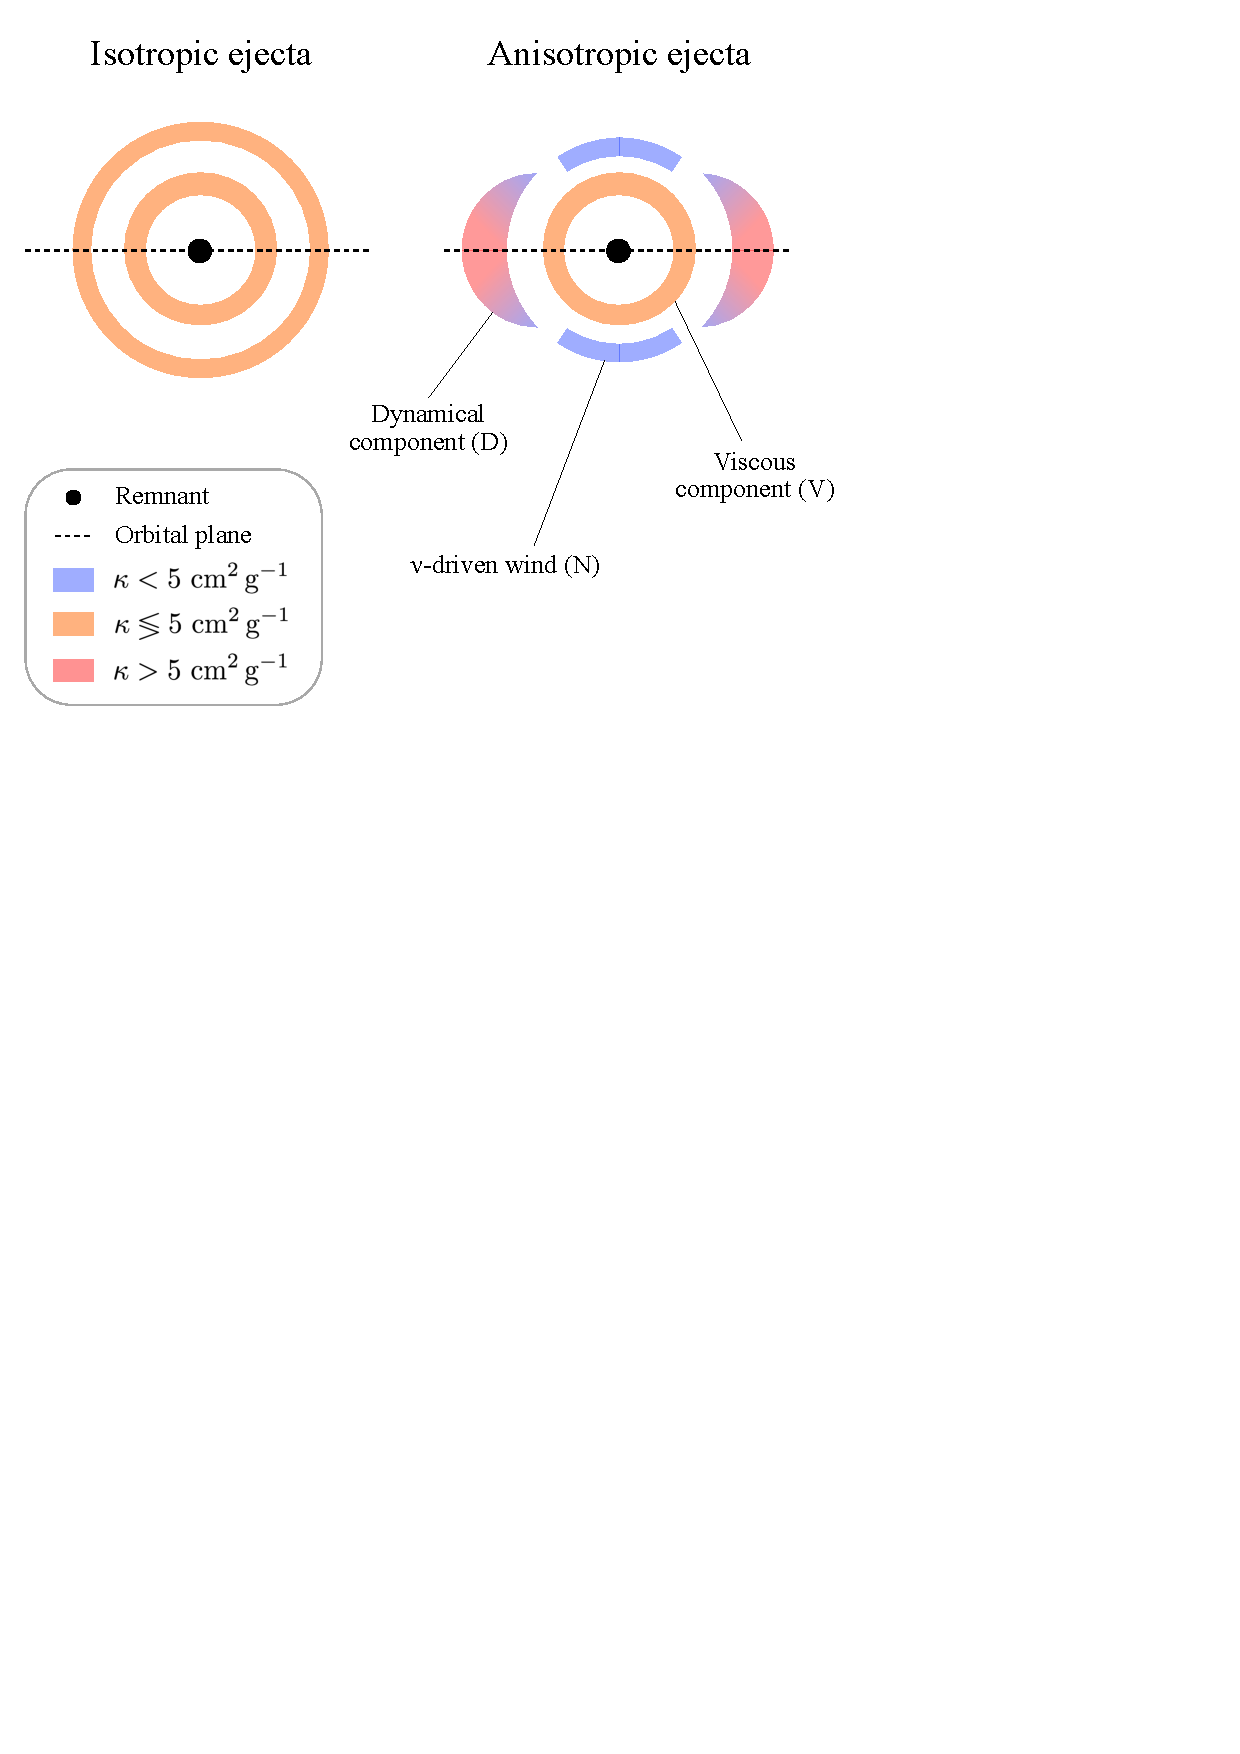
\includegraphics[width=0.58\textwidth]{profiles_op.pdf}
    \caption{Graphic representation of the analyzed
        ejecta profiles for isotropic and anisotropic cases
        from an azimuthal perspective and for a fixed moment of time.
        The black dot represents the remnant and the dashed line is the projected orbital
        plane of the binary. The shadowed areas describe the ejecta profiles: the shape
        characterizes the mass distribution, while the colors refer to 
        the prior assumptions on the opacity parameter.
        In particular, blue regions denote opacities lower than $5~\igscm$,
        red regions refer to opacities greater than $5~\igscm$,
        and oranges areas indicate a broadly distributed opacity.
        All shells are isotropically expanding with a constant velocity.
        (Adapted from \citet{Breschi:2021wzr})
    }
    \label{fig:cartoon}
\end{figure}


For a neutron-rich ejecta, $Y_e\leq 0.2$, the heating rate is dominated by a large statistical 
ensemble of nuclei, however at higher $Y_e\gtrsim 0.2$ corrections are required. 
The time-dependent nuclear heating rate $\epsilon_{\text{nuc}}$ 
%\red{assert notations} 
can be approximated via an analytic fitting formula, derived from detailed nucleosynthesis 
calculations~\citep{Korobkin:2012uy}  
%
\begin{equation}
\label{eq:kilonova:eps_korob}
\epsilon_{\text{nuc}}(t)= \epsilon_0 \, \frac{\epsilon_{\text{th}}(t)}{0.5} \, \epsilon_{\text{nr}}(t) \,
\left[ \frac{1}{2} - \frac{1}{\pi} \arctan\left(\frac{t-t_0}{\sigma}\right)\right]^{\alpha}\,,
\end{equation}
%
where $\sigma = 0.11\,$s, $t_0 = 1.3\,$s, $\alpha=1.3$,
$\epsilon_0$ is the constant and 
$\epsilon_{\text{th}}(t)$ is the 
thermalization efficiency tabulated according to \citet{Barnes:2016umi}.
%
The heating factor $\epsilon_{\text{nr}}(t) $ is introduced as in \citet{Perego:2017wtu} to roughly adjust 
the Eq.~\eqref{eq:kilonova:eps_korob} tp the regime of mildly neutron-rich 
matter (characterized by an initial 
electron fraction $Y_e \gtrsim 0.25$), \citep[see, \eg][]{Martin:2015hxa}, 
%
\begin{equation}
\label{eq:epsnr}
\epsilon_{\text{nr}}(t,\kappa) = \left[1-w(\kappa)\right] + w(\kappa)\,\epsilon_{Y_e}(t)\,,  
\end{equation}
%
where $w(\kappa)$ is a logarithmic smooth clump function such that $w(\kappa < 1~\igscm) = 1$ and 
$w(\kappa > 10~\igscm)=0$ and the factor $\epsilon_{Y_e}(t)$ accounts for the dependency on $Y_e$:
if $Y_e < 0.25$, then $\epsilon_{Y_e}(t)=1$, otherwise, when $Y_e \ge 0.25$,
%
\begin{equation}
\label{eq:epsye}
\epsilon_{Y_e}(t) =\epsilon_{\text{min}}+{\epsilon_{\text{max}}}{\left[1+ e ^{4(t/t_\epsilon-1)}\right]}^{-1}\,,
\end{equation}
%
where $t_\epsilon = 1~{\text{day}}$, $\epsilon_{\text{min}}=0.5$ an $\epsilon_{\text{max}} = 2.5$.

%%%% --------------
% Opacity 
%%%% --------------
%
The mean plank opacities for the hot ejecta are adopted from the systematic study 
(see Figure.~4 in \citet{Tanaka:2019iqp}).
%Notably, the atomic opacity depends on its ionization state. %\red{might reference Barns work}.
When temperature drops and atoms become neutral, the photon opacity sharply decreases. 
This was shown to have a strong effect on 
\acp{LC} in high-frequency bands, \eg, $V$, $U$, $B$ and $g$ \citep{Villar:2017oya}. In order to account 
for the drop in opacity when the temperature falls below the certain value that corresponds to the full 
recombination, the $T_{\text{floor}}$ is introduced \citep{Kasen:2017sxr,Kasen:2018drm} as a minimum value that 
$T_{\text{eff}}$ can have. Due to the presence of lanthanides in the ejcta, 
we consider two floor temperatures, 
depending on the composition: the $T_{\text{floot}}^{\text{Ni}}$ and $T_{\text{floot}}^{\text{La}}$ for 
the lanthanides free and rich ejecta respectively.

%----  EATS integrator
The emission coming from the different angular bins is combined to obtain the spectral flux at the observer location as, 
%
\begin{equation}
\label{eq:spectral_flux}
F_{\nu}(\mathbf{n},t) = \int_{\mathbf{n}_{\Omega} \cdot \mathbf{n}> 0} 
\left( \frac{R_{\text{ph}}(\Omega,t)}{D_L} \right)^2  B_{\nu}(T_{\text{eff}}(\Omega,t))~\mathbf{n} \cdot  \dd\boldsymbol{\Omega}\, , 
\end{equation}
%
where $\mathbf{n}$ is the unitary vector along the line of sight, $\mathbf{n}_{\Omega}$ is the unitary 
vector spanning the solid angle $\Omega$, $D_L$ is the luminosity distance, $R_{\text{ph}}$ is the local 
radial coordinate of the photospheric surface, and $B_{\nu}(T_{\rm eff})$ is the spectral radiance at 
frequency $\nu$ for a surface of temperature $T_{\text{eff}}$. 
%
% ---- Magnitudes
We also make use of the apparent AB magnitude mag$_b$ in a given photometric band $b$, defined as:
%
\begin{equation}
\label{eq:mag}
\text{mag}_b(\mathbf{n},t) = -2.5 \log_{10}\left( F_{\nu_b}(\mathbf{n},t) \right)-48.6\,,
\end{equation}
where $\nu_b$ is the effective central frequency of band $b$.





%% =====================================================================================
%%
%%               R E S U L T S
%%
%% =====================================================================================

%In the following we perform two types of the analysis (i) the fully \ac{NR}-informed \ac{kN} models, where the the only ejecta components considered, are those found in simulations and (ii) the parametric \ac{kN} models, where we use the analytic ejecta profiles, with the parameters obtained from fitting formulae (see Ch.~\ref{ch:stat_anal}).

\begin{figure}[t]
    \centering
    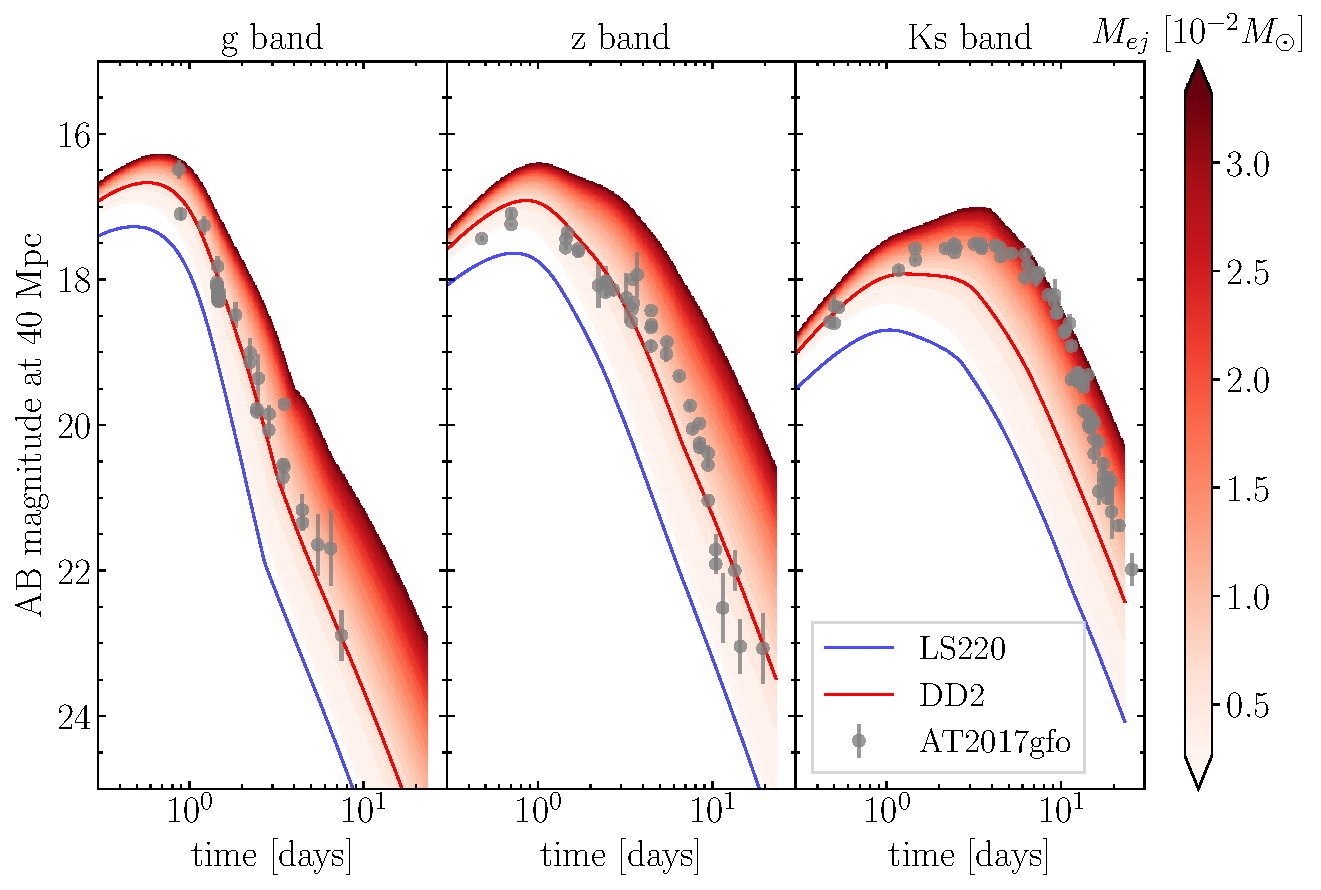
\includegraphics[width=0.75\textwidth]{kilonova/mkn_dd2_band.pdf}
    \caption{Bolometric kN light curves in three representative bands from blue to
        infrared for the two simulations with turbulence viscosity compared to
        \AT{} data from~\citep{Villar:2017wcc}.
        The color gradient is the effect related to different
        \ac{SWW} masses, that suggests possible variations of the light
        curves for different \ac{BNS}. The band is computed by extracting the
        \ac{SWW} mass from DD2 every $10$~ms until the end of the simulation, and
        then by linearly extrapolating the data to $250$~ms.
        (Adapted from \citet{Nedora:2019jhl})
    }
    \label{fig:knlc}
\end{figure}


\section{\ac{SWW} for the blue component of \AT{}}\label{sec:kilonova:result}

The \ac{BNS} merger ejecta consists of several anisotropic components with different 
properties (see the discussion in Sec.~\ref{sec:intro:ejecta} and Chapter~\ref{ch:bns_sims}).
%
%Hence, the \ac{kN} model ought to account for the anisotropy of the ejecta composition. Additionally, the interaction between components needs to be included, but we leave this to future works.
%% ---
Indeed, outflow properties inferred for \AT{} using multi-components and 2D \ac{kN} models including the ejecta anisotropy and cross-component irradiation are broadly compatible with the results from simulations, \eg, \citep{Kawaguchi:2018ptg}, see also Sec.~\ref{sec:intro:kilonova}. 
%% ---
The particular challenge however, is to reproduce the early blue emission. 
Both semi-analytical and radiation transport
models require ejecta properties different from those found in
simulations. In particular, 
this component requires fast low opacity, massive ejecta \citep{Fahlman:2018llv} that is generally 
not found in \ac{BNS} simulations.
%% ---
Notably, the early blue component can be explained by the emission arising 
in the interaction between a relativistic jet and the ejecta
\citep{Lazzati:2016yxl,Bromberg:2017crh,Piro:2017ayh}.
However, simulations show that that successful jets do not deposit a sufficient amount of thermal energy in the ejecta for this mechanism to work \citep{Duffell:2018iig}. 
Other possibilities include the presence of highly magnetized winds \citep{Metzger:2018uni,Fernandez:2018kax},
or the presence of the so-called viscous dynamical ejecta \citep{Radice:2018ghv}.
These two explanations require the development of large-scale strong magnetic fields.
%% ---
In this section we show that the presence of the massive \ac{SWW},
found in the ab-initio \ac{BNS} merger simulations with long-lived \ac{NS} remnants 
(see Chapter~\ref{ch:bns_sims}) can help explain the early blue emission, 
relaxing the need for strong ordered magnetic fields. 


We begin by considering two equal mass \ac{NR} \ac{BNS} merger models with LS220 
and DD2 \acp{EOS}, that produce short and long-lived \ac{NS} remnant respectively. 
Using the \texttt{MKN} code, discussed above, we construct \ac{NR}-informed 
\acp{LC} for both, \ac{DE} only and the combination of \ac{DE} and \ac{SWW}\footnote{
    The \texttt{MKN} code does not include the effects of multiple ejecta component 
    iteration. We leave this to future works.
}.
%%% ---
%For both models we produce \ac{NR}-informed \acp{LC}, using both the \ac{DE} and \ac{SWW} for the model with the long-lived \ac{MNS} remnant, and \ac{DE} only for the model with the short-lived one.
%% ---
The result is shown in Fig.~\ref{fig:knlc}.
We observe, that the \ac{DE} only is insufficient to explain the \AT{} in 
all bands considered irrespective of the \ac{BNS} model. However, the informed 
by both \ac{DE} and \ac{SWW} \ac{LC} of the DD2 $q=1.00$ (\texttt{SR}) model 
is sufficiently bright to account for the emission in 'z' band. 
%% However, it appears dimmer than the early blue \AT{} emission in 'g' band. 
%% ---
The emission in low frequency bands requires a more massive 
\ac{SWW} with mass ${\gtrsim} 2\times10^{-2}M_{\odot}$, implying a remnant lifetime of ${\gtrsim}200$~ms, as the \ac{SWW} mass flux is present as long 
as \ac{MNS} remnant is present (see Sec.\ref{sec:bns_sims:mj_loss}).
However, a more massive \ac{SWW} is incompatible with
the early emission for the low-frequency bands of \AT{}.
%% --- 
In order to explain the late emission in the low frequncy bands and 
early emission in high frequency bands, a combination of the \ac{SWW} and 
viscous ejecta from the disintegration of the disk are required.
%% --- 
Our results, however have uncertainties related to our simplified calculation of
the \ac{kN} \acp{LC} which is expected to be less accurate at
late times when absorption features and deviations from \ac{LTE} become more relevant \citep[see \eg][]{Smartt:2017fuw}.
To model the \ac{kN} emission more robustly, the time- and energy-dependent 
photon radiation transport models are required 
\citep{Kasen:2017sxr,Tanaka:2017qxj,Miller:2019dpt,Bulla:2019muo}.
Additionally, the systematic uncertainties in
nuclear (\eg, mass models, fission fragments and $\beta$-decay
rates) and atomic (\eg, detailed wavelength dependent opacities for
\rproc{} element) physics enter all the current \ac{kN} models 
\citep{Eichler:2014kma,Rosswog:2016dhy,Gaigalas:2019ptx}.




%\subsection{Conclusion}
%
%\red{Copied}
%Standard kN models applied to the early AT2017gfo light curve are in
%tension with ab-initio simulations conducted so far.
%While alternative interpretations have been proposed, they are either
%disfavored by current simulations and observations (e.g. jets) \citep{Bromberg:2017crh,Duffell:2018iig},
%or require the presence of large-scale strong magnetic 
%fields which might not be formed in the postmerger
%\citep{Metzger:2018uni,Fernandez:2018kax,Radice:2018ghv,Ciolfi:2019fie}. 
%We identified a robust dynamical mechanism for mass ejection that
%explains early-time observations without requiring any fine-tuning.
%The resulting nucleosynthesis is complete and produces all
%$r$-process elements in proportions similar to solar system abundances.
%Methodologically, our work underlines the importance of employing
%NR-informed ejecta for the fitting of light-curves.
%Further work in this direction should 
%include better neutrino-radiation transport and magnetohydrodynamic effects
%\citep{Siegel:2017nub,Fujibayashi:2017puw,Radice:2018xqa,Radice:2018pdn,Miller:2019dpt}. 


\section{Fit-informed kilonova models}


%% KILONVA PLOTS
\begin{figure*}[t]
    \centering 
    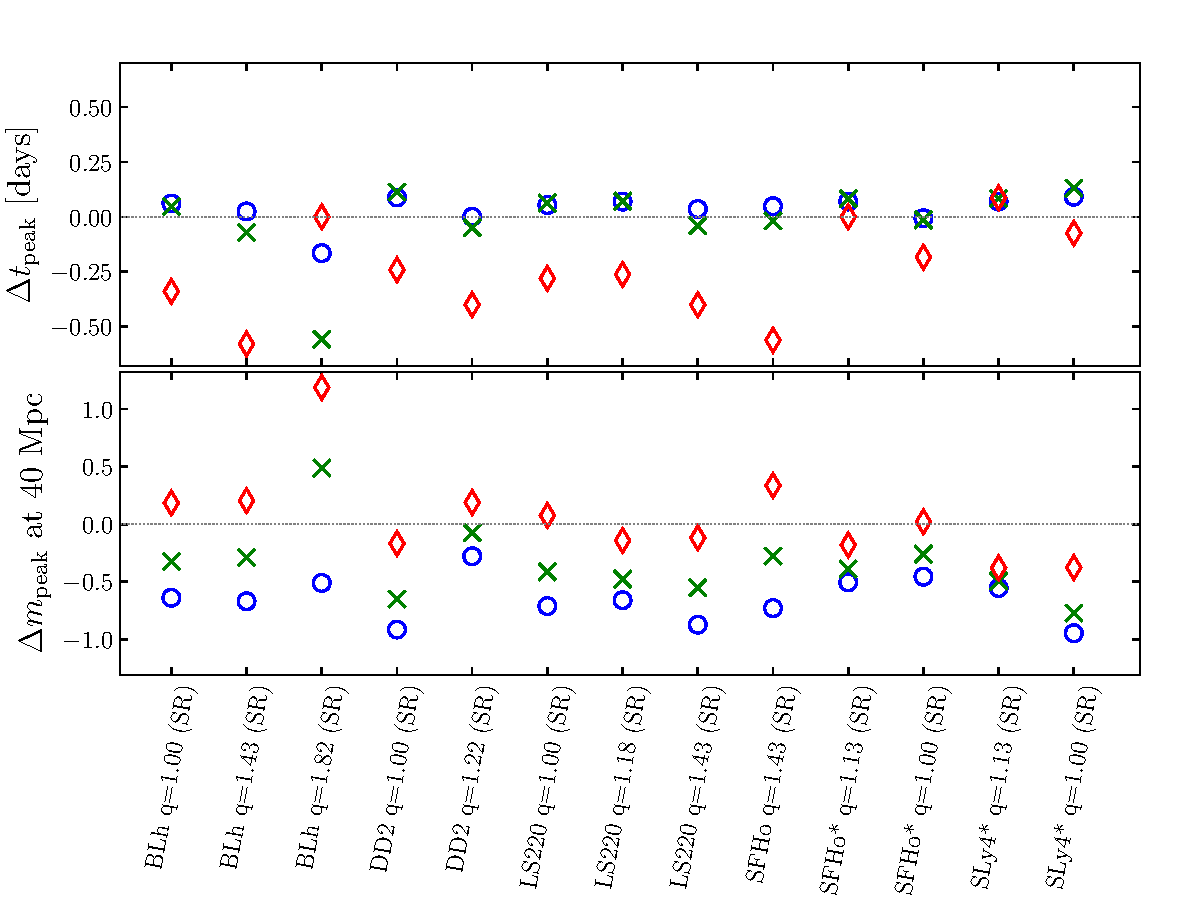
\includegraphics[width=0.49\textwidth]{kilonova/mkn_multiband_dyn_NR.pdf}
    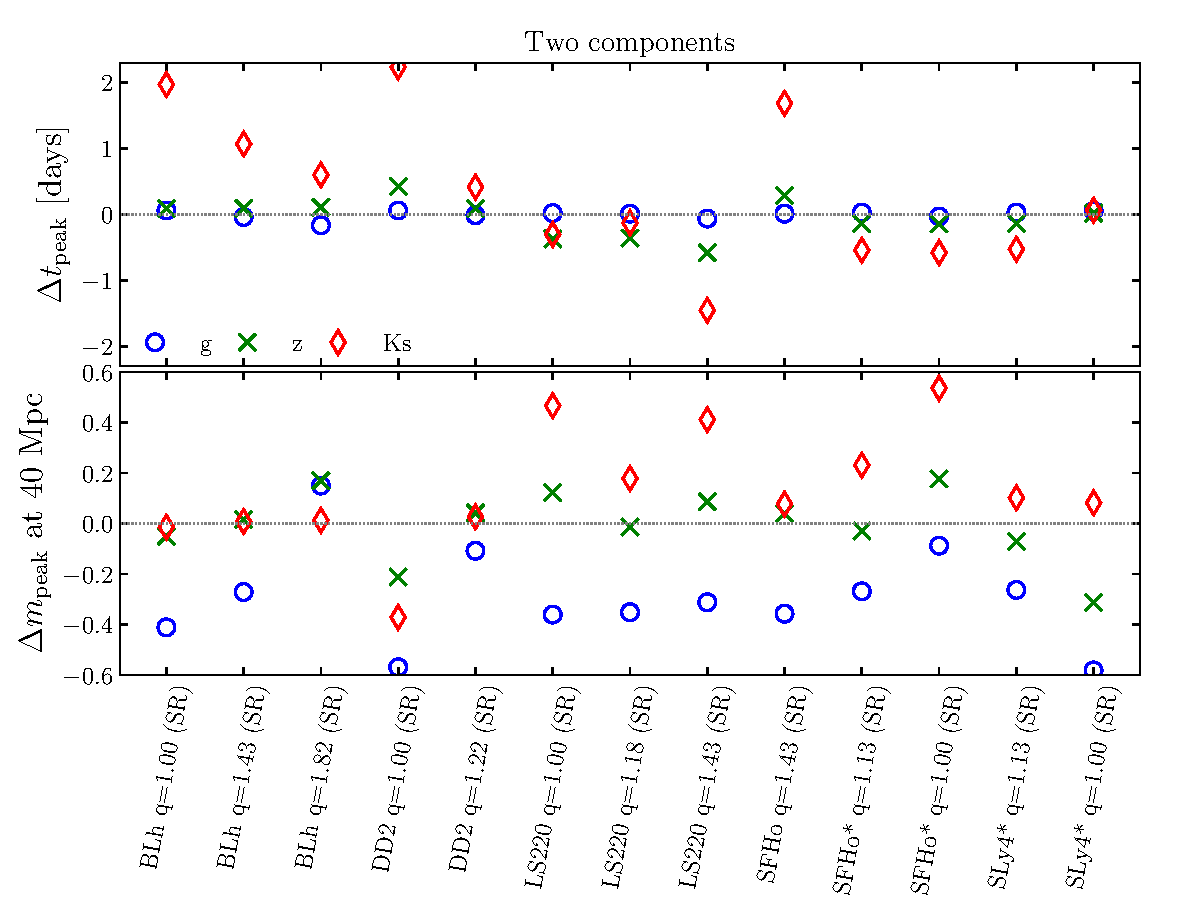
\includegraphics[width=0.49\textwidth]{kilonova/mkn_multiband_dynsec_NR.pdf}
    \caption{
        Comparison between one component light curves (\textit{left panel}) and
        two components light curves (\textit{right panel}) in $g$, $z$ and $K_s$
        bands using direct NR input or the fitting formulae for the
        dynamical ejecta and disk mass. 
        The $y-$axis displays the difference between the peak time 
        (\textit{top panel}), $\Delta t_{\rm peak} = t_{\rm peak; NR} - t_{\rm peak; fit}$, 
        and peak magnitude, $\Delta m_{\rm peak} = m_{\rm peak; NR} - m_{\rm peak; fit}$, 
        (\textit{bottom panel});
        the $x-$axis shows selected BNS models of \DSrefset{}.
        The fits employed here are the polynomials in $(q,\tilde{\Lambda})$ used with the 
        best fitting coefficients, calibrated to \DSheatcool{} (that includes \DSrefset{}).
        The plot shows that 
        the light curves generated with the dynamical ejecta fits (one
        component) tend to underestimate the peak times and magnitudes
        of NR-informed light curves, especially in the $K_s$ band. In case of 
        dynamical ejecta and disk wind (two
        components) light curves, the peak
        time is less constrained ($\pm 2$~days) in the $K_s$ band, but the
        peak magnitudes is predicted more accurately $\pm0.5$~mag. }
    %% \vn{Note! That for NR-informed lightcurves \textbf{full} NR ejecta profile (for dyn. ej.)
    %% is fed into MKN. Thus here the geometric effects and poor fit performance contribute to the
    %% qdeviation.}
    \label{fig:mkn_example}
\end{figure*}

%In this section we investigated statistical properties of the \ac{DE} and remnant from 
%several sets of \ac{NR} \ac{BNS} models. 
%
%The analysis showed that the properties of the ejecta and remnant disk mass are subjected 
%to large systematic uncertainties that stem from difference in input physics: neutrino 
%treatment and \ac{EOS}.
%%
%Additionally, we assessed the performance of different fitting formulae to the ejecta 
%parameters, such as mass, velocity, electron fraction and \ac{RMS} half-opening angle, 
%and the disk mass. We noted that the formulae that include explicitly $\tilde{\Lambda}$ 
%and \mr{} are able to capture the leading trends. Specifically, the simple second order 
%polynomial, $P_2^2(q,\tilde{\Lambda})$ performs on par or better than more complex 
%fitting formulae in terms of $\chid$.
%%
%However, all fits are characterized by large $\chid$. That suggests that either the 
%error measures we adopt are too strict, or more complex fitting formulae are required. 
%We leave this investigation to future works, when larger sample of \ac{NR} \ac{BNS} 
%models with advanced physics is available.
%%
%%We stress that while these fits, provide an important links between the binary parameters 
%%and the properties of \ac{EM} counterparts, useful for \ac{MM} studies 
%%%% \citep{Dietrich:2020efo,Breschi:2021tbm,Nicholl:2021abc}, 
%%they have to be used with caution, specifically, as some fitting formulae suggested in the 
%%literature give ill-constrain fits.
%%% --- 
%
%Because of its simplicity and overall best (in comparison) performance, we recommend 
%the second order polynomial in $q$ and $\tilde{\Lambda}$, (the Eq.~\eqref{eq:polyfit22}).
%For its calibration we suggests datasets with the most advanced physics, \ie, 
%\DSrefset{} and \DSheatcool{}.
%The calibration for polynomial fits are given in Tab.~\ref{tab:dynfit:poly} for ejecta 
%and in Tab.~\ref{tab:diskfit:poly} for the disk. The recommended calibration is 
%highlighted with gray in the tables.
%We refer to this fits as ``best fitting formulae'' hereafter.
%
%
%The best fitting formulae are able to reproduce the ejecta velocity to to ${\sim}50\%$ with 
%$68\%$ significance range being $(-0.4,0.2)$. The electron fraction is recovered with the 
%${\sim}0.1$ error margin and the \ac{RMS} half-opening angle is -- with ${\sim}10$~deg
%error margin.
%The masses of the \ac{DE} and of the remnant disk are more uncertain and can be faithfully 
%reproduced only within the order of magnitude and a factor of a few respectively. 
%While this is a very large error margins, we note, that this is an improvement with 
%respect to the previous studies \citep[\eg][]{Dietrich:2016fpt}.
%%% ---

%Overall, we find that rather simple fitting formulae are able 
%to fit the data on par or better then more complex fitting formulae available in the 
%literature that also can provide an ill-constrain fits.
%The ejecta and remnant properties are subjected to large uncertainties, that in part 
%are due to different physics input: neutrino treatment and \acp{EOS}.
%Specifically, as the neutrino reabsorption is a crucial component for the reliable 
%estimates of the \ac{DE} mass 
%\citep[\eg][]{Wanajo:2014wha,Sekiguchi:2015dma,Perego:2017wtu,Foucart:2018gis},
%it is highly important to enlarge the \DSheatcool{} and reasses the ejecta properties statistics. 
%%
%Additionally, sets of \ac{NR} models with different chirp masses would allow to asses 
%new trends in data.

%% --- Kilonova
Fitting formulae to the ejecta and remnant parameters are often used to predict the 
properties of the \ac{EM} counterparts to mergers and to infer the properties of the 
binary from the observations of \ac{EM} counterparts, often as a part of \ac{MM} studies 
\citep{Dietrich:2020efo,Breschi:2021tbm,Nicholl:2021rcr,Dietrich:2020efo}.
%
In Ch.~\ref{ch:bns_sims} Sec.~\ref{sec:bns_sims:ejecta}, we pointed out that the 
simple polynomials in \mr{} and $\tilde{\Lambda}$ provide a reasonable fit to 
ejecta properties of \ac{BNS} mergers. 
%
%
%
%However, it is important to acknowledge the limitations that these simple 
%fitting formulae have, and that we outlined in the sections above. 
%
Here we compare the properties of the \ac{kN} \acp{LC} informed by these fitting 
formulae and by the ejecta profiles from \ac{NR} simulations presented in 
Ch.~\ref{ch:bns_sims} (using the same method as in previous section). %The same method was used in Sec.~\ref{sec:kn:results}
We employ the semi-analytic \ac{kN} model of \citet{Perego:2017wtu} discussed 
above and consider either one or two ejecta components.
%in 
%Ch.~\ref{ch:kilonova} and consider either one or two ejecta components.

When one component \ac{kN} is considered, only the \ac{DE} ejecta properties are used, 
such as mass, velocity, and \ac{RMS} half-opening angle separating the low opacity 
power outflow and high opacity equatorial one. The angular distributions of mass and velocity 
are assumed to be the same as in \citet{Perego:2017wtu}.
When two component \ac{kN} is considered, in addition to the \ac{DE} we model the 
secular outflow from the disk, assuming that a fixed fraction, $40\%$ of it would 
become unbound. The angular distribution of mass, velocity and opacity
is assumed to be uniform. 
Comparing the properties of \ac{NR}-informed and fit-informed \ac{kN} \acp{LC} we 
maintain all the other parameters fixed.
%

The resulted comparison between the peak times, $t_p$, and magnitudes, $m_{\rm AB}$ 
evaluated for three different bands: $g$, $z$ and $K_s$ 
is shown in Fig.~\ref{fig:mkn_example}.
Considering the one-component \ac{kN} \ac{LC}, (left panel), we note that the $t_p$ is 
recovered with the ${\sim}0.2$~days error margin i nthe $g$ and $z$ bands and with a 
$0.5$~days margins in $k_s$ band. Notably, the fit-informed \ac{LK} have a systematically
underestimated $t_p$ in the $K_s$ band. 
The largest deviation is found for the model with \mr{} of $1.8$ and BLh \ac{EOS}.
Comparing the peak magnitudes, $m_{\rm AB}$ we observe that the difference 
between the \ac{NR}- and fit-informed \acp{LC} is on average ${\sim}0.5$~mag. 
In $b$ band, however, the deviation is ${\sim}1$~mag.
Considering the two-component \ac{kN} models (right panel), we observe that the 
$t_p$ in the $K_s$ band differ between the fit- and \ac{NR}-informed \acp{LC} by 
${\sim}2$~days. The $m_{\rm AB}$ is reproduced within the ${\sim}\pm 0.5$~mag in $z$ 
and $K_s$ bands.
The larger difference between the $m_{\rm AB}$ for one compoent \ac{kN} \acp{LC} lie 
in the influence of the ejecta geometry that is not fully accounted for by a single 
$\athetarms$ parameter that we use to separate low and high opacity material. 
%
Overall, we note that while exact reasons of the deviations can be attributed to 
the exact \ac{LC} model employed, this example suggests that the minimum systematic 
variations are to be expected in synthetic \acp{LC} informed by our best fitting formulae.
